\chapter{Generation of Seed Light}\label{generationOfSeedLight}

In this chapter, we will discuss the design and construction of the Master Laser. 

\section{Stabilization of Master Laser}
\subsection{Master Laser Layout}
The Master Laser is a 408 nm extended cavity diode laser(ECDL). It consists of a laser diode mounted in a temperature-controlled housing from the Thorlabs LDM21 family of products. It is collimated by a small, aspherical lens (Thorlabs C570TM-A). A picture of the master laser can be seen in Fig.\,\ref{master_laser_photo}, while a picture of the inside of the housing can be seen in Fig.\,\ref{master_laser_interior_photo}.

\begin{figure}
\centerline{
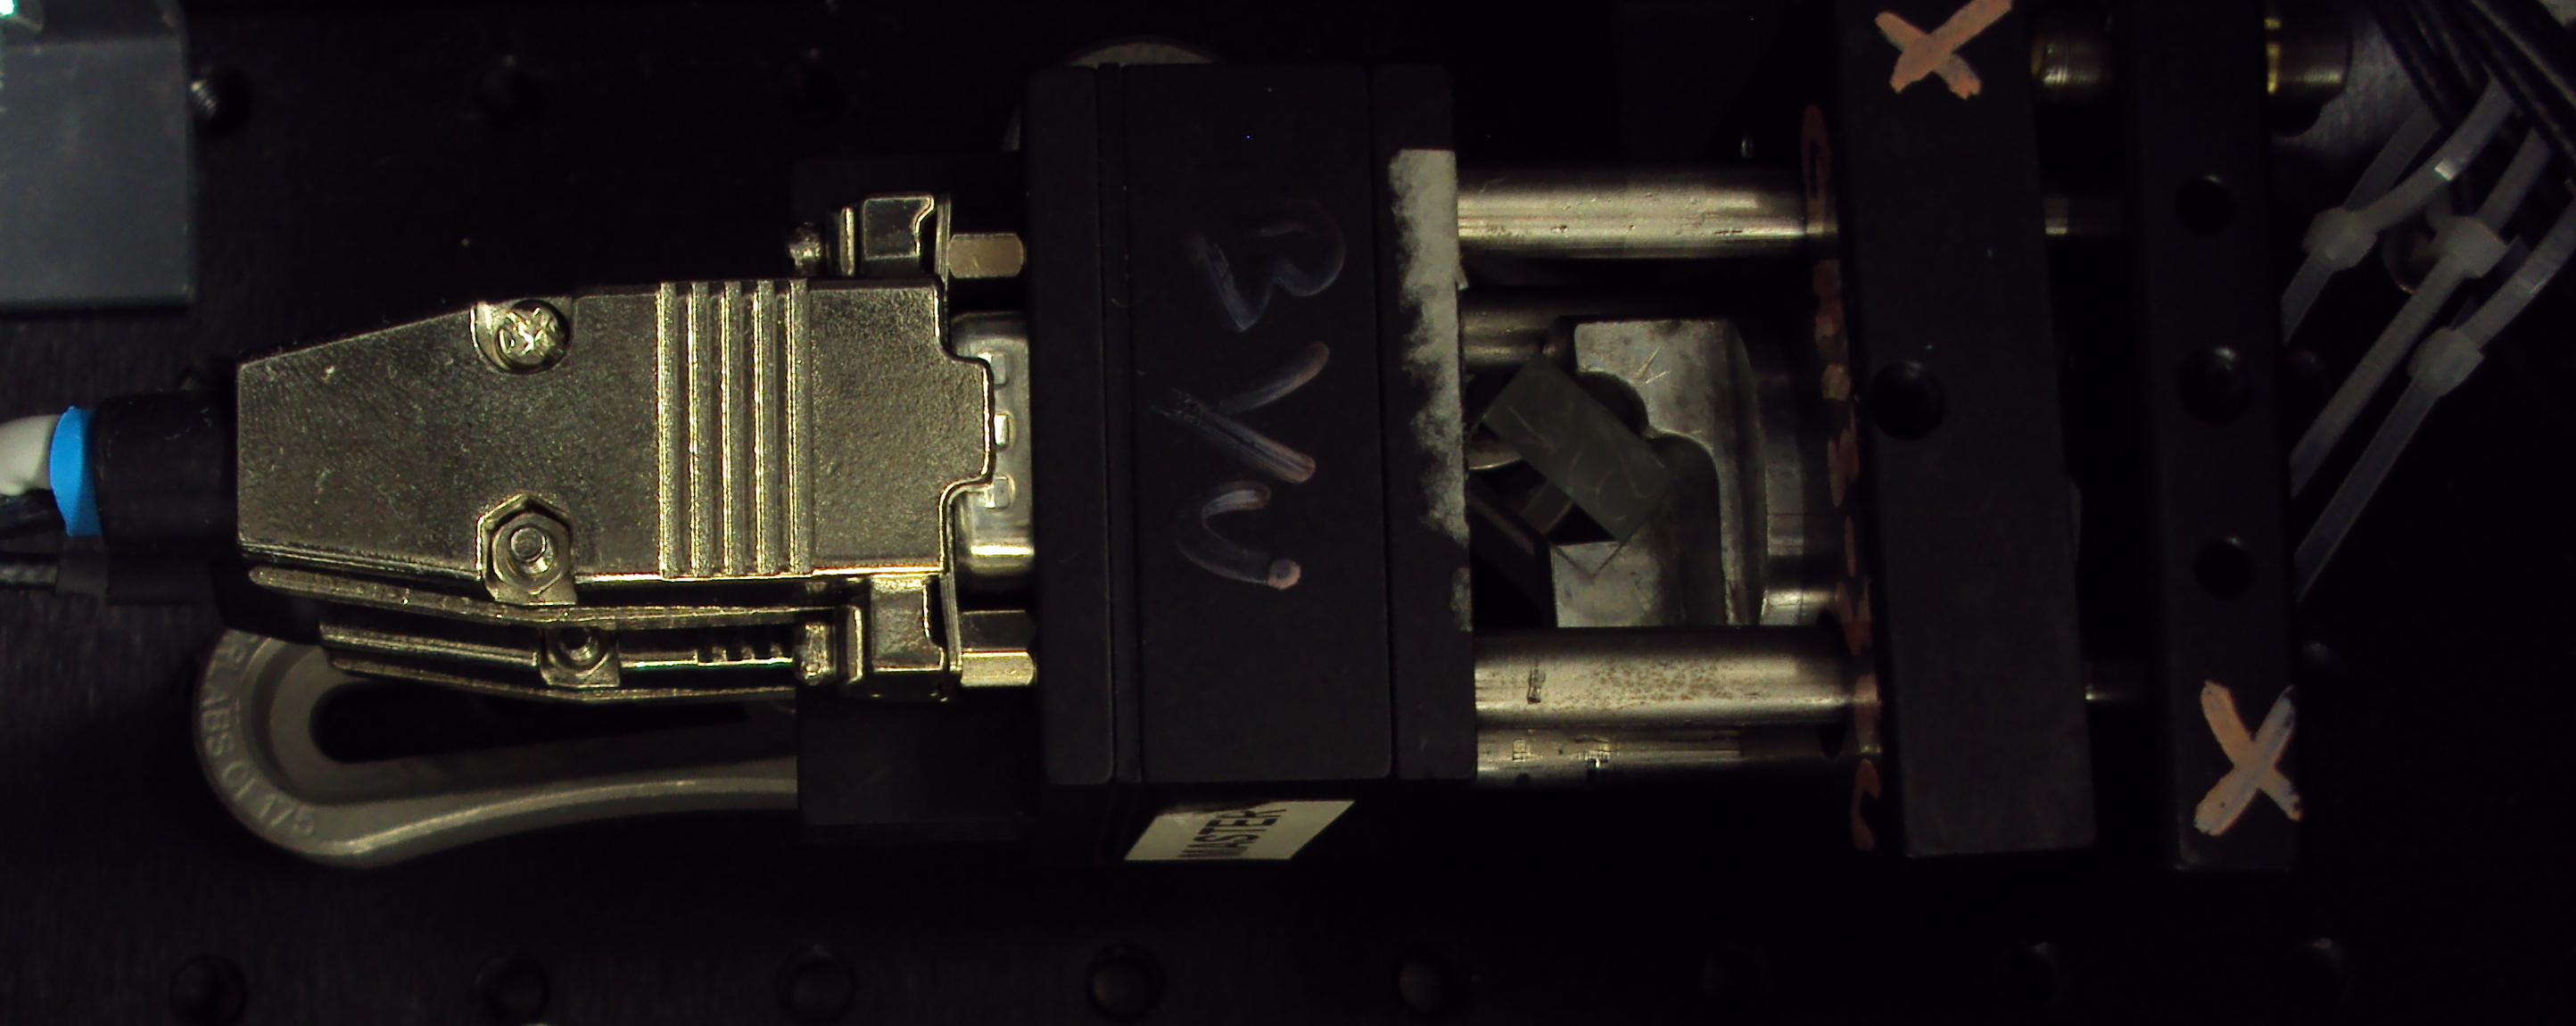
\includegraphics[width=0.95\textwidth]{master_laser.JPG}}
\caption[Photograph of Master Laser]{\label{master_laser_photo} The master laser is housed in the black box in the upper right of the picture. The diffraction grating that is used for feedback is mounted on a custom mount close to the Master Laser aperture. We initially tried several other configurations. However, after several iterations, we found that the use of the metal rods to provide direct  mechanical coupling between the laser and grating mount were necessary for stable single-mode operation. We also found through trial and error that the distance of $\sim$4 cm seemed to work. }
\end{figure}

\begin{figure}
\centerline{
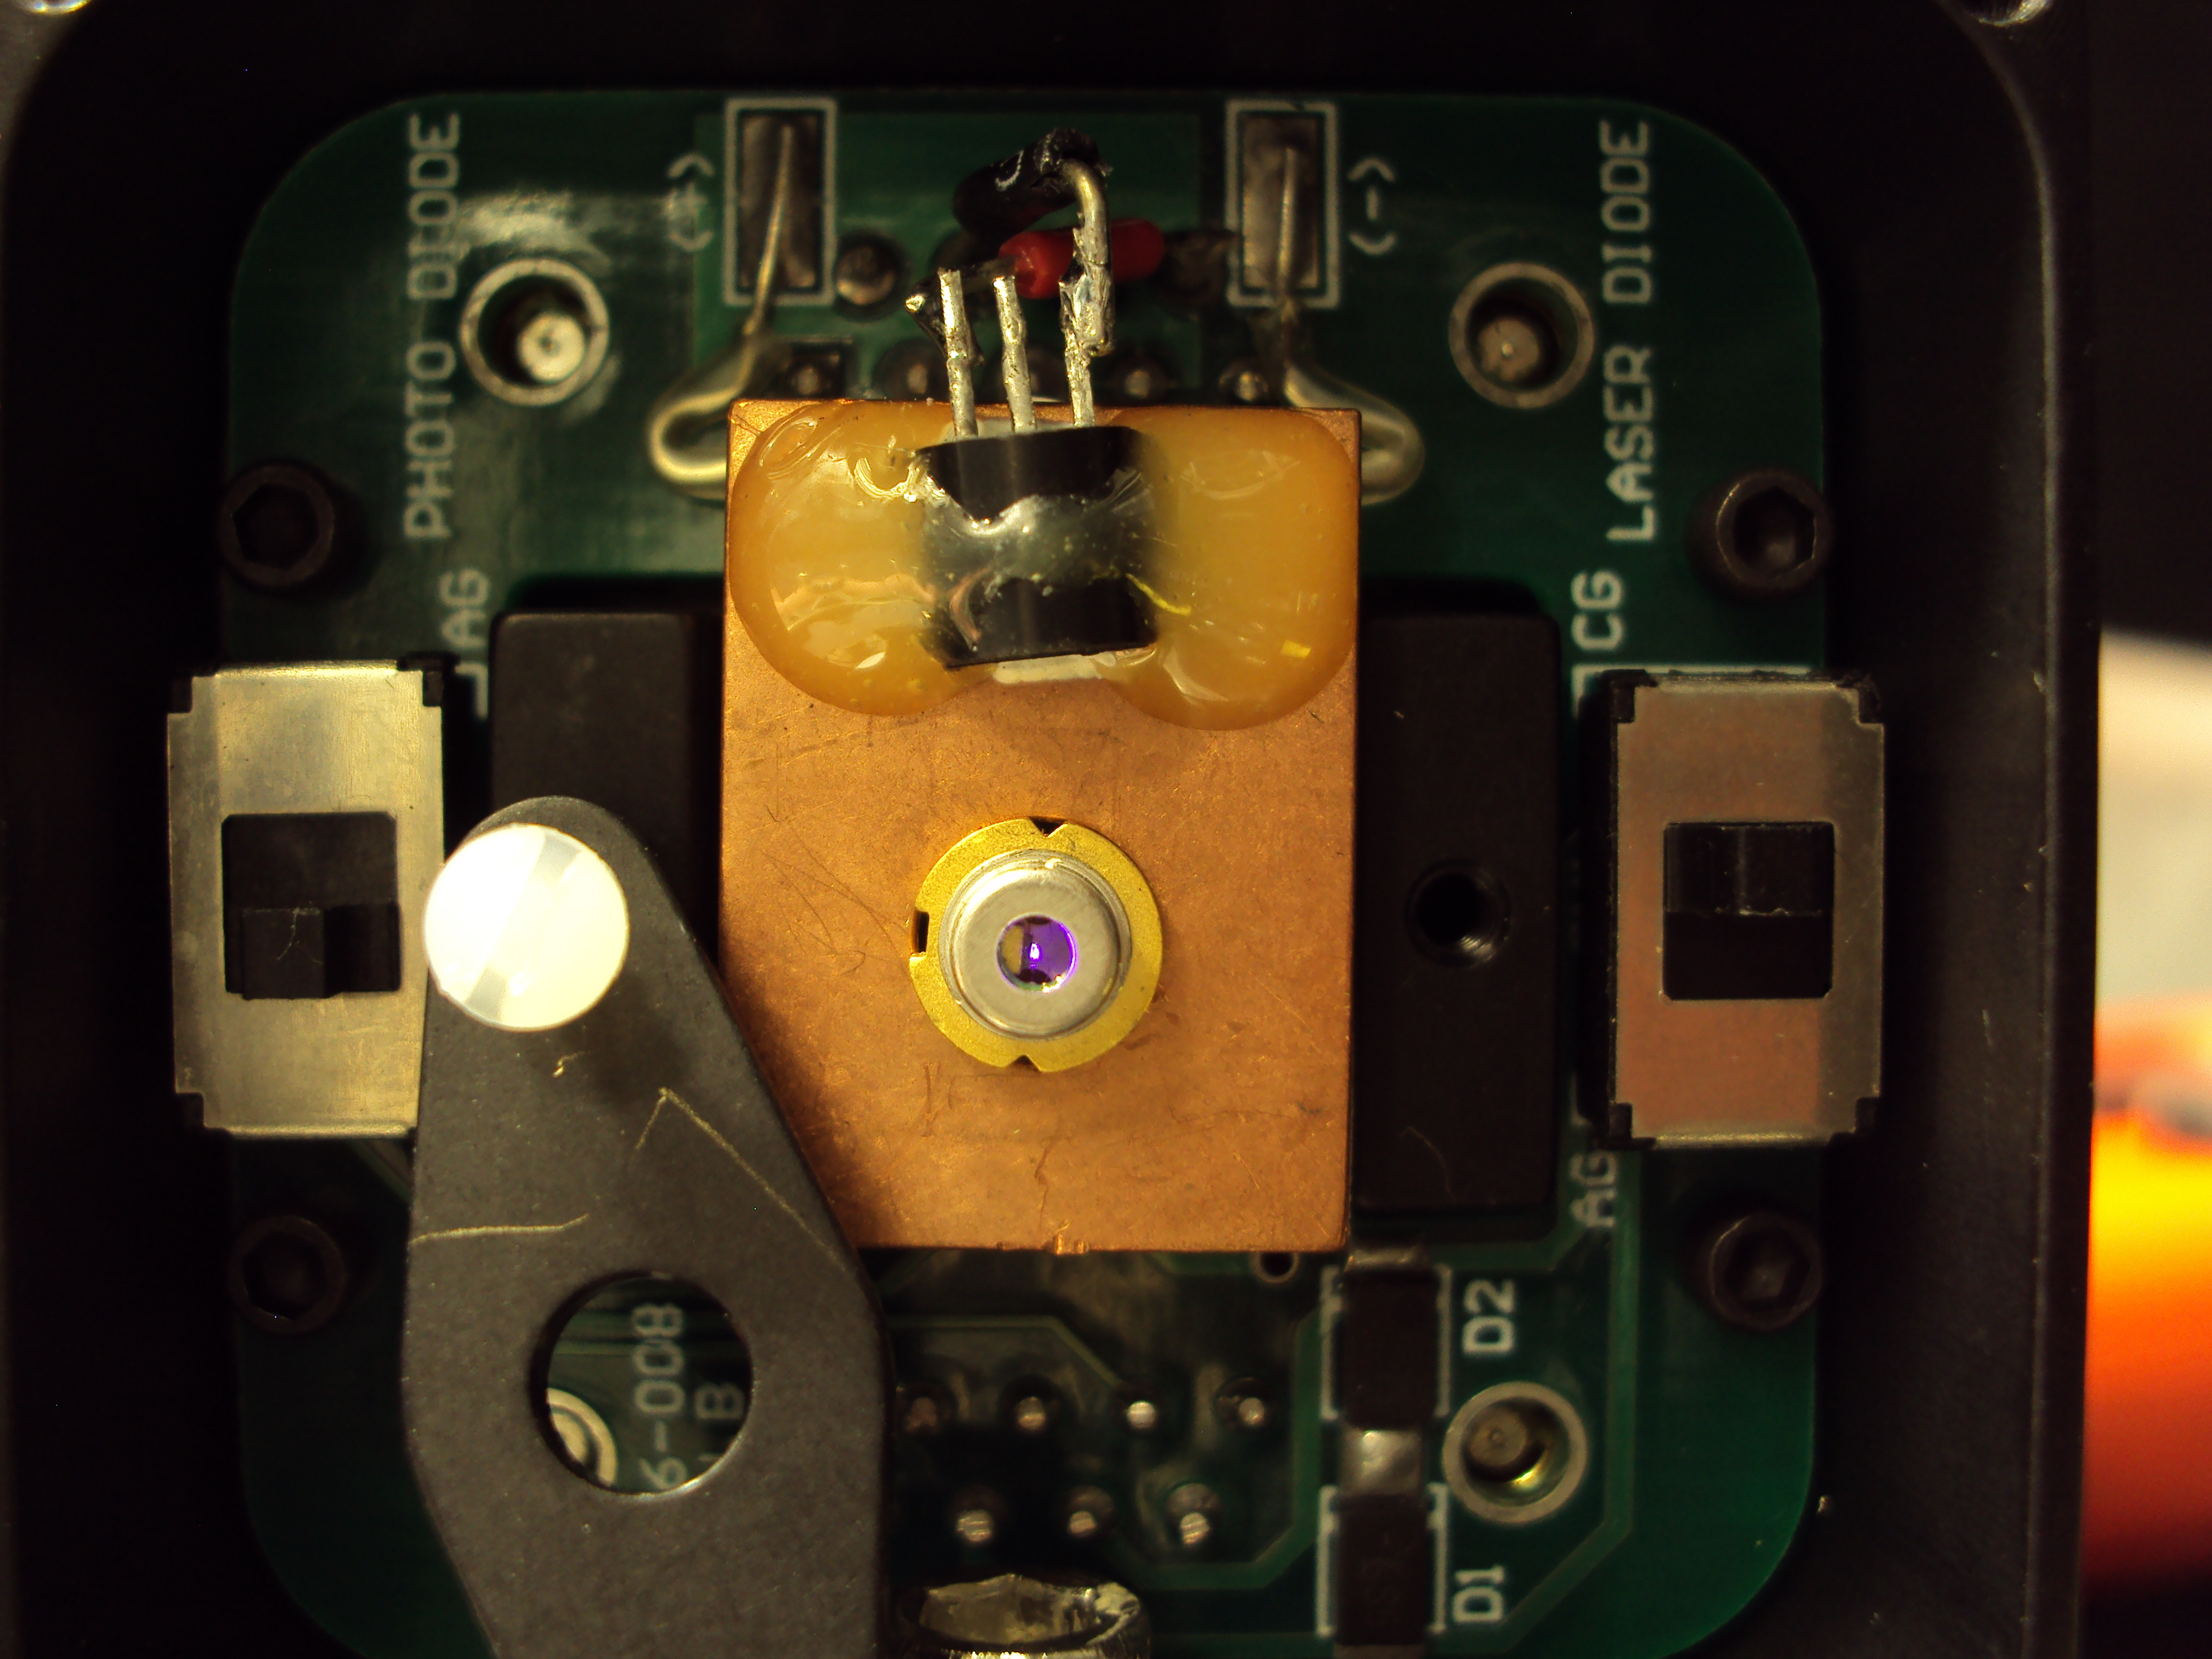
\includegraphics[width=0.95\textwidth]{laser_on_in_housing.JPG}}
\caption[Photograph of Master Laser Diode]{\label{master_laser_interior_photo} The Master laser in its housing. We modified the housing to include an additional temperature sensor (the AD592), which can be seen glued to the top of the copper plate.}
\end{figure}
%why did we do the rods? Do I have it in my notes?

\subsection{Master Laser Diodes}
The diode used in the master laser is a single-spatial mode InGaN diode that is very similar to the diode lasers used in Blu-ray players. 

The diode in the master laser is a Mitsubishi ML320G2, which was wavelength-selected by the distributor (i.e. the distributor performed measurements and binned the parts based on their output wavelengths; we then ordered lasers from their 408 nm bin).
As backup diodes, we also bought 30 diodes on eBay that had been removed from Blu-ray or HD-DVD players and measured their wavelengths in order to bin them ourselves. Some of these diodes were ultimately used in the slave lasers.

We initially tried to build the Master laser using a non-wavelength-selected Sharp GH04020A2GE low power diode, which we could not stabilize for unknown reasons. We quickly switched to a non-wavelength-selected Sharp GH04P21A2GE diode for the Master laser. However, this laser's free-running wavelength at 25$^\circ$C was far too low. In order to tune this diode to the correct wavelength, we found that we had to maintain the diode at a temperature of $\sim$60$^\circ$C. This resulted in degradation of the diode and loss of power over the course of a few months.

\subsection{Grating Spectrometer Wavelength Measurements}

In order to tune the Master laser to precisely the correct wavelength and to measure the room temperature free running wavelength of the uncharacterized lasers (i.e. the lasers that were bought on eBay and later used in the slave lasers), we used a compact grating spectrometer from the Ocean Optics USB2000 series to measure the center frequency of the bare laser diodes. This spectrometer uses a diffraction grating to separate light based on its constituent wavelenghts. Light scattered off the diffraction grating is detected by a CCD array consisting of 2048 pixels that is also enclosed in the spectrometer. The average difference in wavelength between adjacent pixels is $\sim$.061 nm. % This according to /research/octave/ooSpectrumData12Sep/MasterFile.m using the lambdas variable defined in there.

We tried to maximize the resolution and accuracy of our measurements. The center wavelength of the bare diodes changed only a few nanometers over the entire range of possible temperatures and currents. In order to ensure accurate absolute wavelength measurements, we calibrated to a mercury source both before and after looking at the spectra of the various lasers. We feel confident in our calibrations since Mercury conveniently has spectral lines at 405 and 436 nm, which are close to our target wavelength of 407.771 nm. A typical before and after calibration spectrum taken using the Mercury lamp can be seen in Figure\ref{calibrationData}. When analyzing the peaks produced by the laser on the grating spectrometer, we fit the measured data to a Gaussian distribution in hopes of squeezing out some sub-pixel level resolution of the peak location. Examples of this type of analysis are shown in Figures\,\ref{Temperaturespectra} and \ref{wavelengthselected}.

We also had a Bristol 521 Wavelength meter, which uses a Michelson-Morley interferometer to measure wavelength. However, for the free-running lasers, we used the spectrometer since the linewidth of the free-running diodes was too large for use with the wavelength meter. 
%diagram of which method to use where? 
%The basic 

%\subsection{Master Laser Temperature and Current Selection}

The temperature and the current of the laser are two of the main means we have for affecting the wavelength of the Master laser. Using a grating spectrometer, we measured the center wavelength of the bare laser (i.e. no grating feedback or extended cavity).


We have data on the wavelength dependence on temperature and current for our laser. This data is plotted in Fig.\,\ref{3dCurrentandTgraph}. We see that the variation of the center wavelength of the laser is linear to a good approximation over reasonable values of temperature and current.

\begin{figure}
\centering
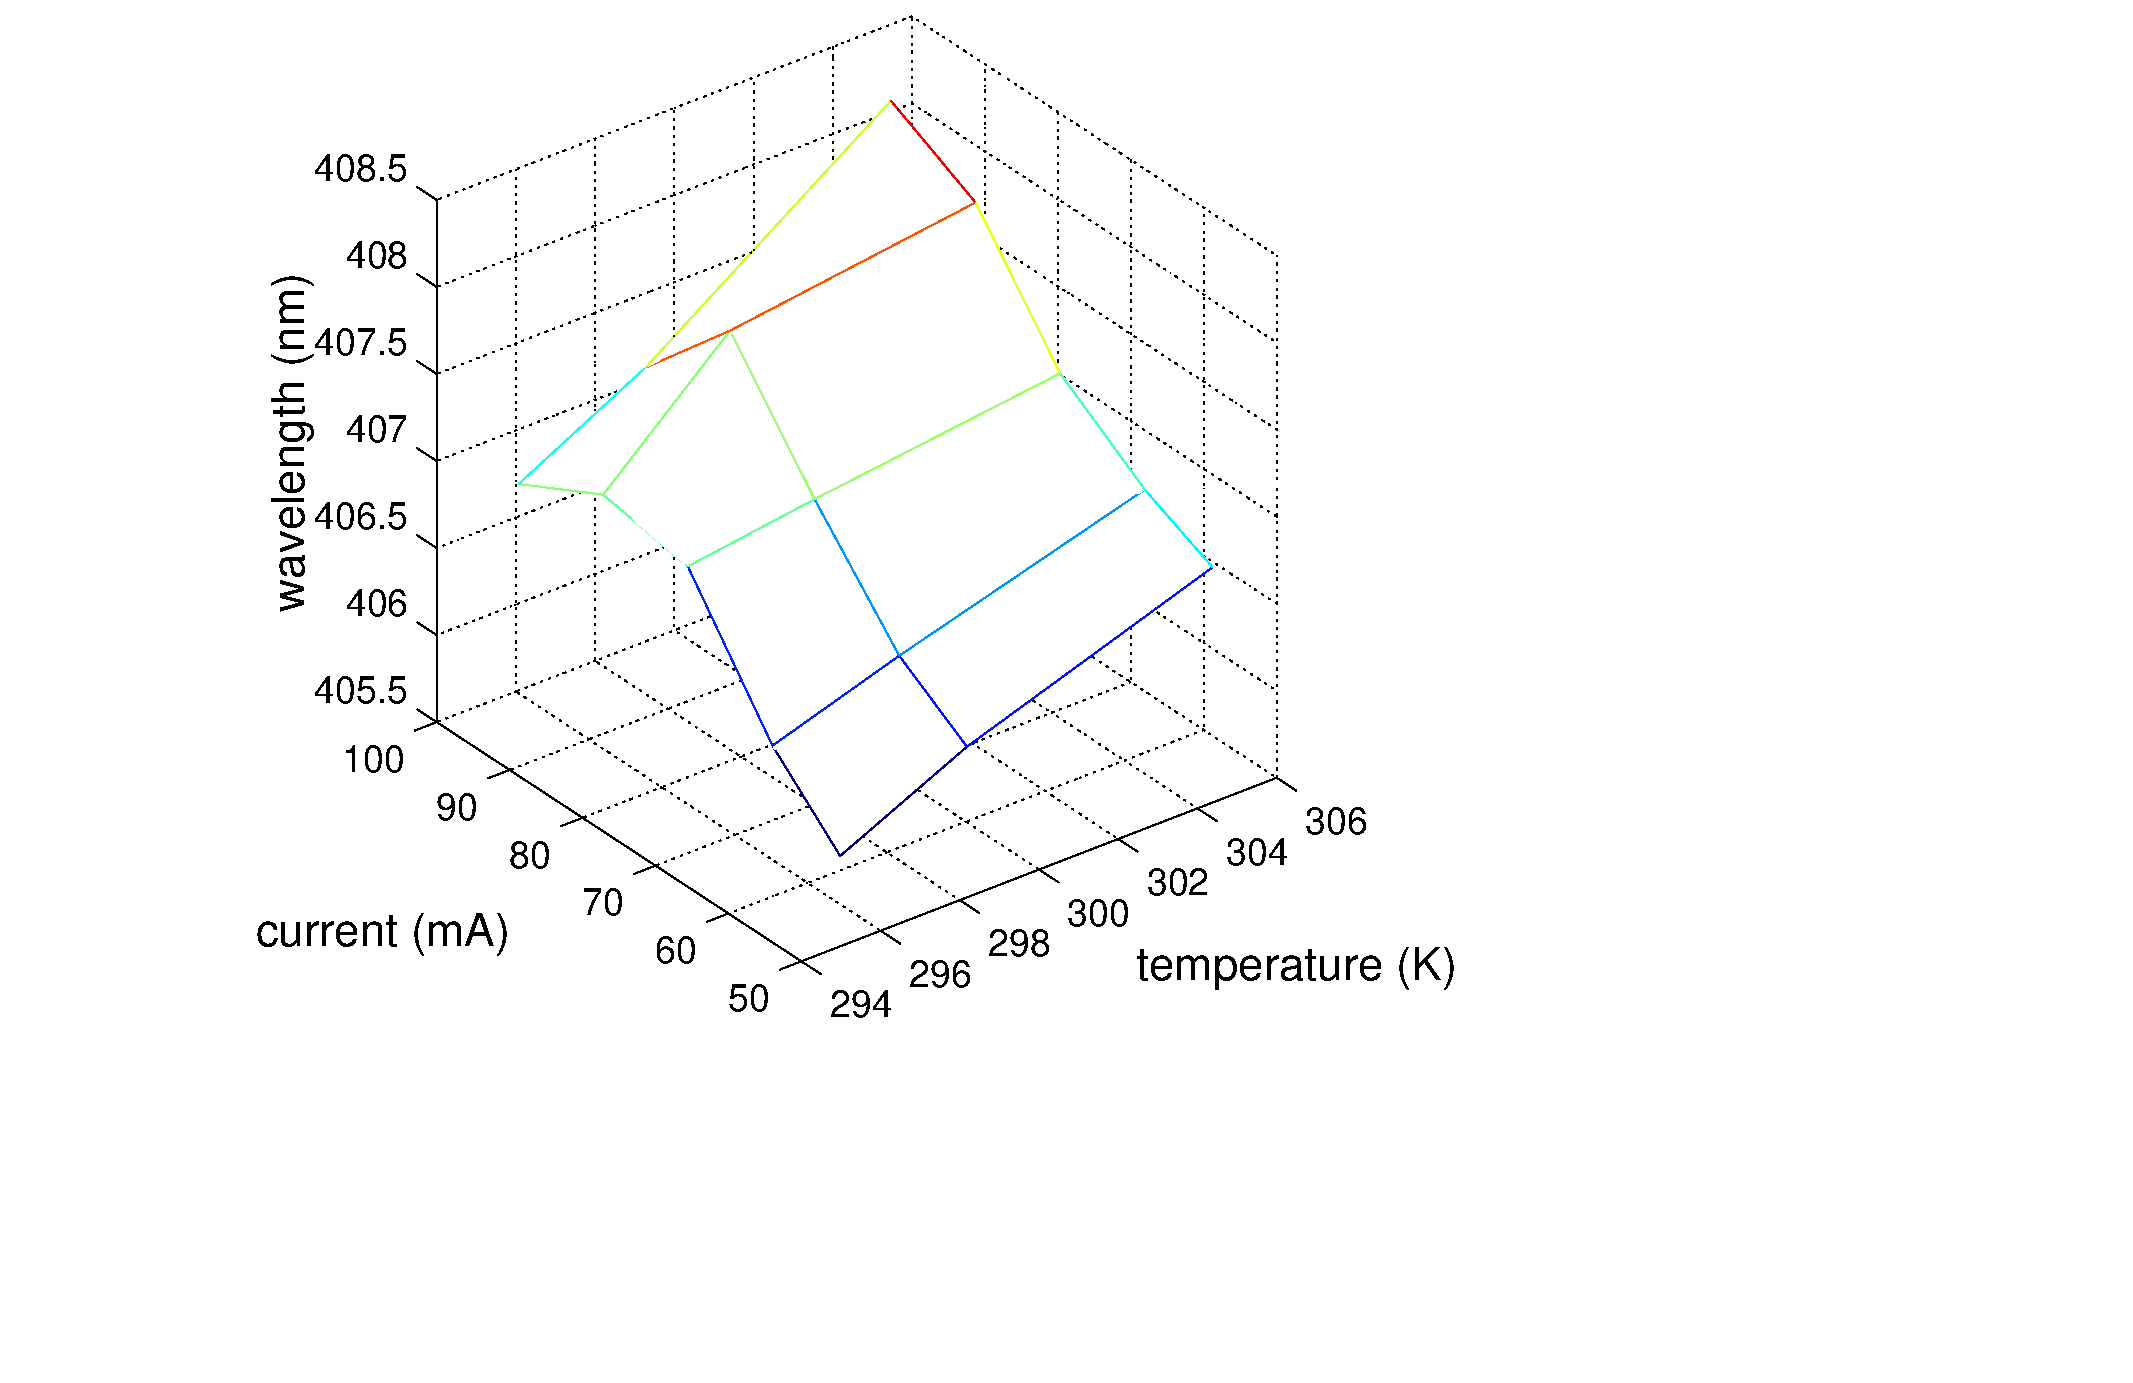
\includegraphics[width=0.7\textwidth]{TVlambda3} 
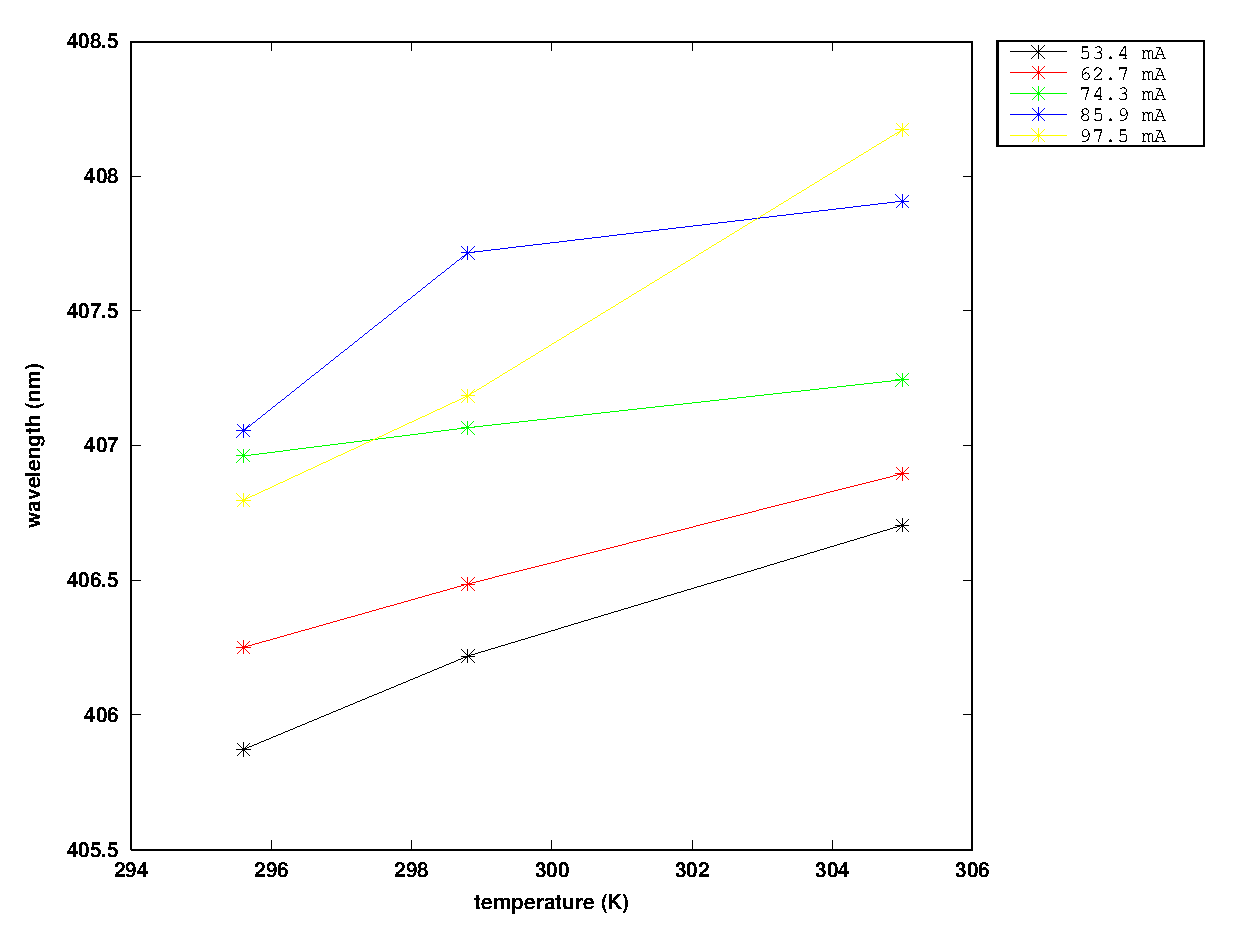
\includegraphics[width=0.7\textwidth]{TVlambda2}
\caption[Graph of Temperatures and Currents]{\label{3dCurrentandTgraph} Representative data of the free-running wavelength of our Master laser as a function of nominal current and nominal temperature.}
\end{figure}
%possibly not the master? ehhh. IDK. 
%\footnote{I have no idea what accounts for the variation between diodes}. 
\begin{figure}
\centering
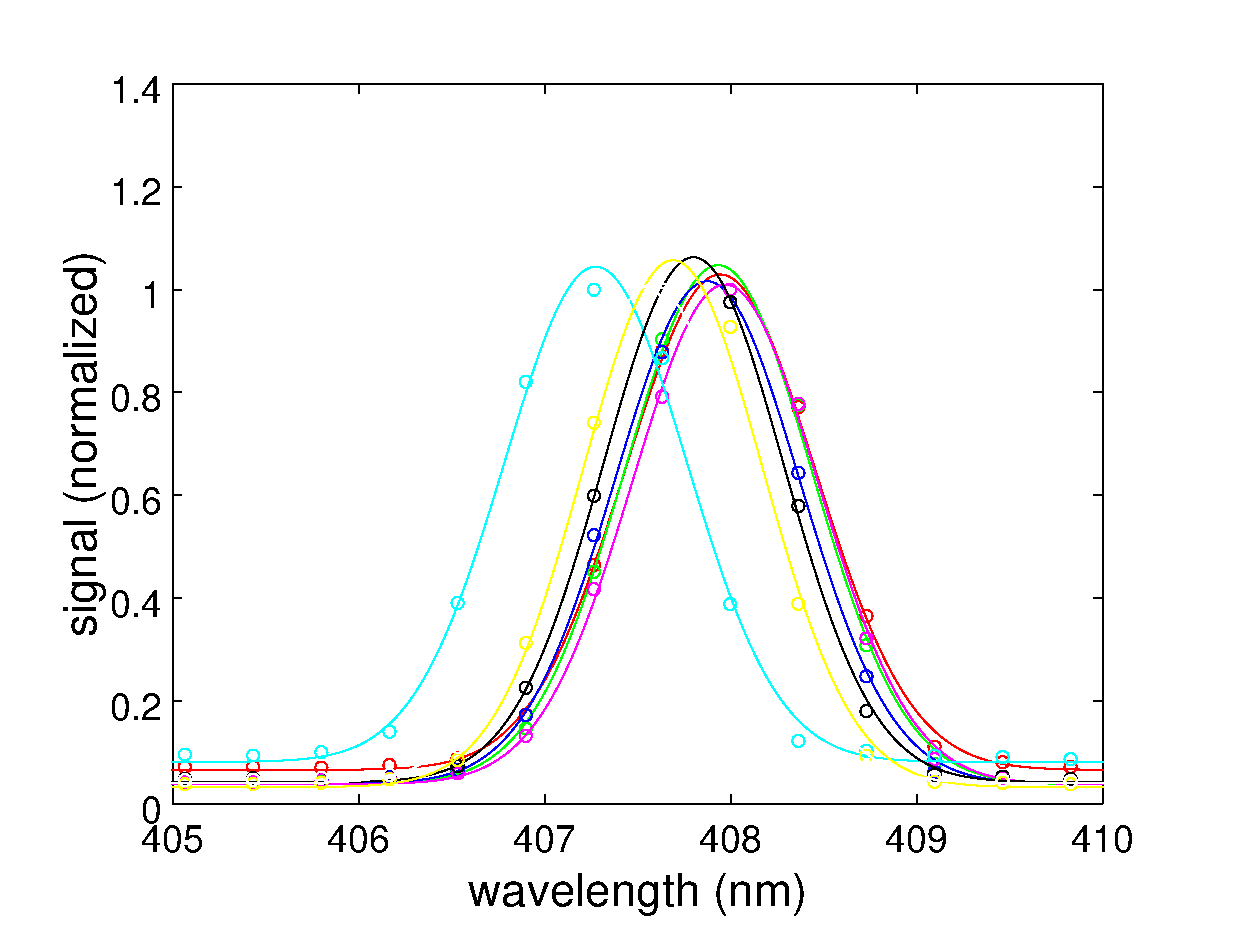
\includegraphics[width=0.95\textwidth]{wavelength_selected} 
\caption[Wavelength selected diodes]{\label{wavelengthselected} Representative data of the free-running wavelength of several wavelength selected lasers taken at 120 mA.} %temperature? %the ones we picked or someone else did? 
\end{figure}
\begin{figure}
\centering
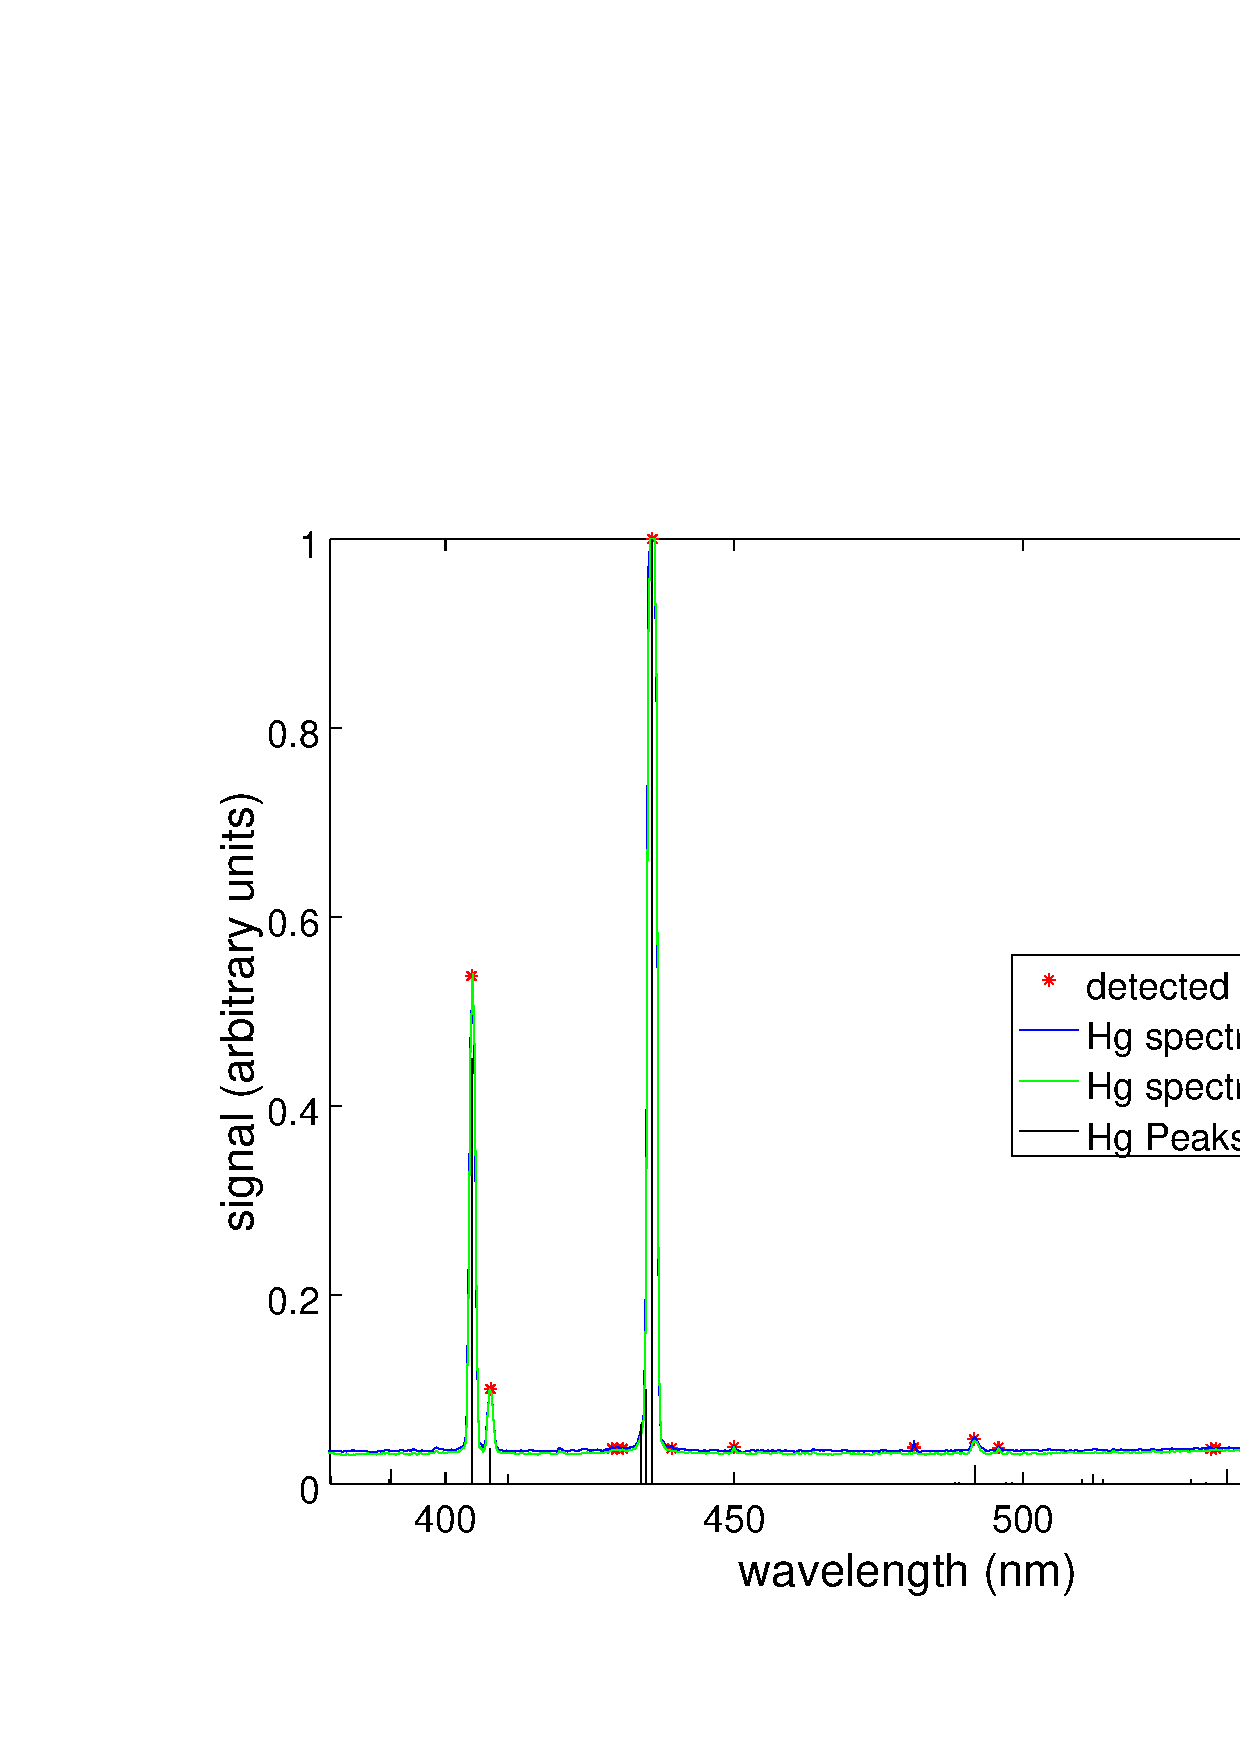
\includegraphics[width=0.95\textwidth]{calibrationData} 
\caption[Calibration spectrum from Hg Lamp]{\label{calibrationData} Data from the calibration using the mercury lamp. We deliberately allowed some of the farther away peaks to saturate in order to improve our signal for the peaks near 408 nm. The black lines represent spectral lines taken from the NIST Atomic Spectra Database\cite{NISTasd}. The detected peaks in measured spectrum refers to the peaks that we found in the measured data from the Hg lamp using Octave}
\end{figure}

\begin{figure}
\centering
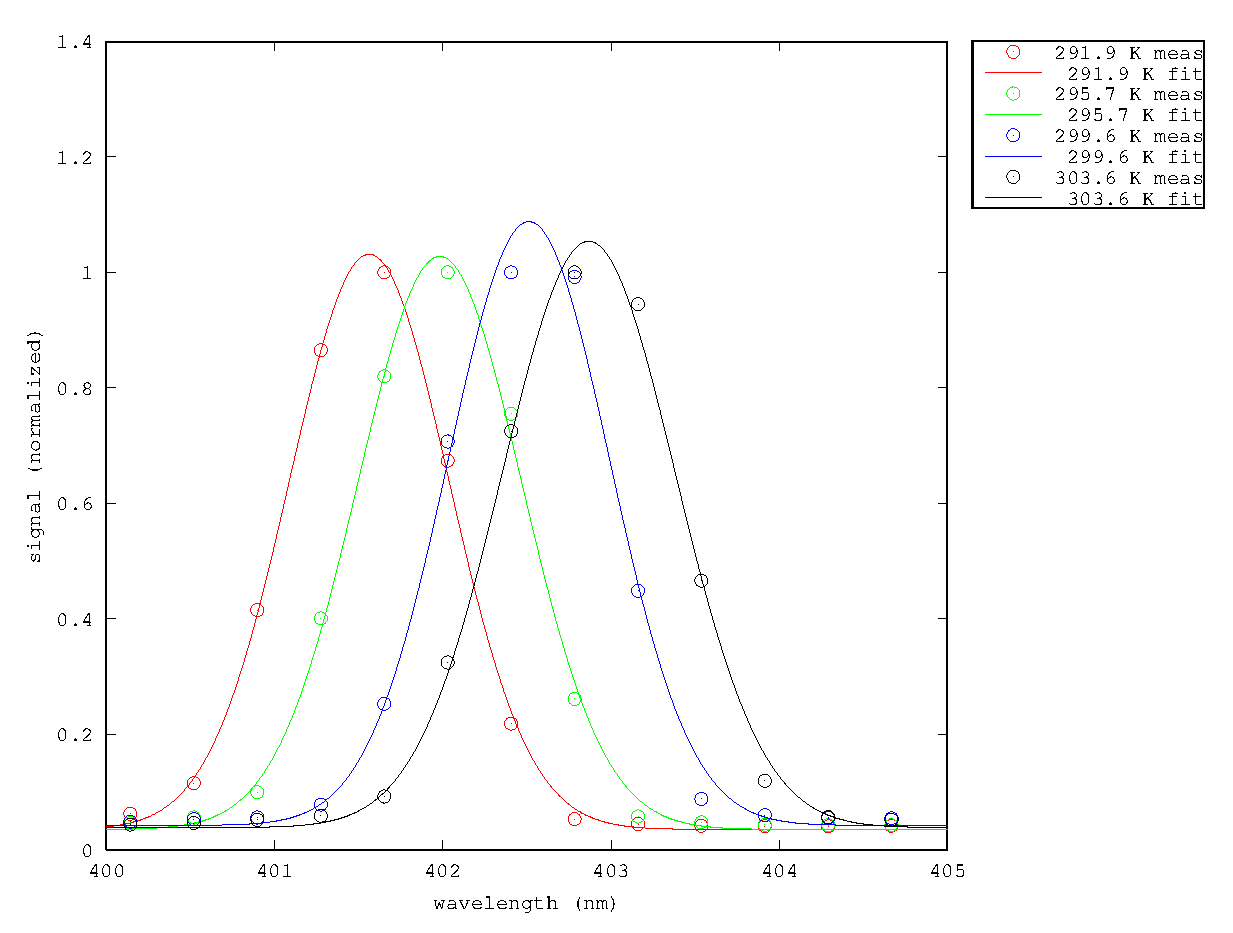
\includegraphics[width=0.95\textwidth]{temperatureFit} 
\caption[Wavelength of Master laser at different temperatures]{\label{Temperaturespectra} Representative data of the free-running wavelength of our Master laser as a function of temperature.}
\end{figure}

\subsection{Placement of the Grating}

%Some theory here might be worth reviewing. In addition, I did that really great mathematica notebook where I calculated all that stuff. 

%Installation of a diffraction grating allows us to selectively couple light of particular wavelengths back into 

Lasers work by amplifying light resonant with a particular mode of the laser cavity via stimulated emission. Ideally, we would like to favor a mode within the diode laser corresponding to our desired wavelength. In order to accomplish this, we add yet another resonant cavity outside our laser that can couple light back into the laser. 

This cavity is formed by a diffraction grating on one side and the entrance of the laser on the other side. This configuration is called an Extended Cavity Diode Laser (ECDL). The grating we selected was a Thorlabs model number GH13-36U, which has 3600 lines/mm. A picture of the grating can be seen in Figure\,\ref{diffractionGratingPhoto}. 

\begin{figure}
\centerline{
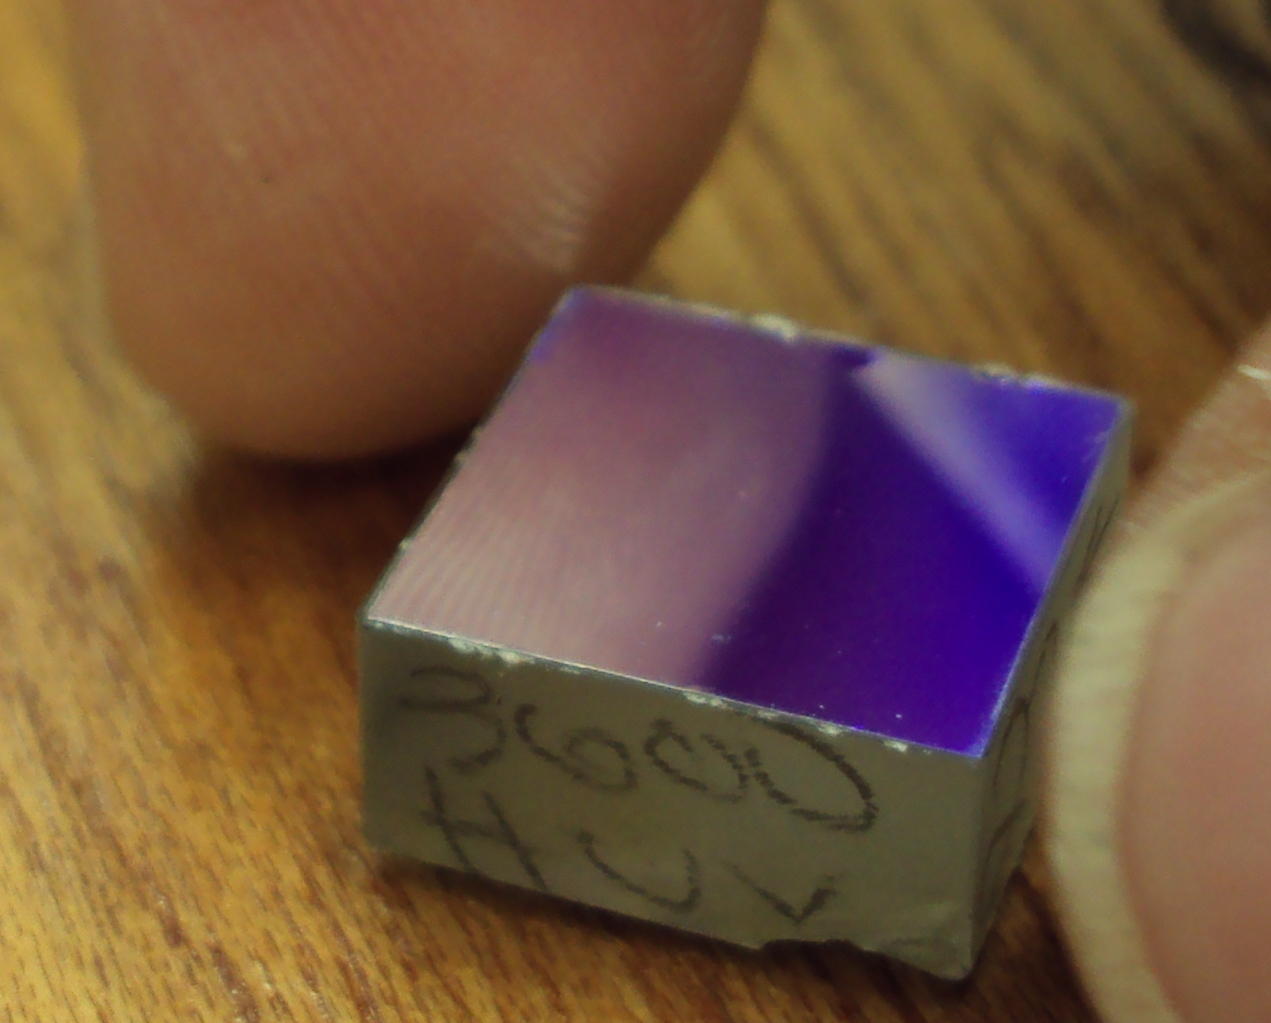
\includegraphics[width=0.95\textwidth]{diffractionGrating.JPG}}
\caption[Photograph of Diffraction Grating]{\label{diffractionGratingPhoto} The diffraction grating before it is installed.}
\end{figure}

The diffraction grating is angled so that the first order diffraction peak at 407.771 nm light is directed back into the laser. The condition for this to be the case is 

\begin{equation} \label{gratingEQn}
n \lambda = 2 d \sin (\theta),
\end{equation}

where $n$ is the order of the diffraction peak (in our case, $n=1$), $d$ is the spacing between slits (in our case $d=1 mm/3600 = 278 nm$) and $\theta$ is the angle of incidence to the grating. We can therefore calculate that the $\theta$ should be approximately
\href{http://www.wolframalpha.com/input/?i=arcsin%28+407.771+nm+%2F%282*%281+mm%2F3600%29%29%29+in+degrees}{$47.2^\circ$}.

 We machined a custom grating holder out of Aluminum, which can be seen in Figure\,\ref{master_laser_photo}. The aluminum holder was mounted in a Thorlabs piezoelectric mount, which allows us the necessary fine control of the grating's location and angle over a narrow range of angles.  The grating was mounted approximately 4 cm from the aperture of collimating lens.
% The grating is mounted at such an angle that it selectively couples light with a wavelength near 408 nm back into the laser cavity. The resonant space between the diffraction grating and the collimating lens is what the phrase ``extended cavity'' refers to. The additional boundary conditions imposed on the resonant modes of the laser by the external grating result in a narrowing of the laser's linewidth. 
 We must ensure that the diffraction grating is installed such that both the angle and the cavity length match our desired wavelength. In order to get the grating aligned initially, we turned on the current to the laser until the laser was just below the threshold where it would begin lasing. We then aligned the grating using the threaded actuators on the piezoelectric mount until we saw the output power of the laser increase. When this happens, it indicates that we are successfully coupling light to the laser cavity. The output power of the laser can be monitored by eye or by instrument and it is fairly easy to get a feel for what it should look like when the grating first couples to a laser operating just below threshold.

%did I ever tune it to the right wavelength using the Bristol wave meter? 
In order to stimulate the transition, the master laser must also be tunable over some range. Therefore, the piezoelectric actuators can be connected to control circuitry that can be used to tune the laser based on a signal derived from transmission through a Strontium vapor cell. 

The control circuitry will consist of a simple PID controller similar in design to the PID controllers used elsewhere in the lab \cite{cjeDiss}. The vapor cell will produce a signal from which we can derive an error signal. The PID controller takes the error signal and produces a feedback signal. This feedback signal can then be used to control the voltage on the piezoelectric actuators along with the current to the laser. The PID controller's output stage allows the user to select various gains that control the movement of each of the piezoelectric actuators. 
%did I ever tune this up? 

We would like to discuss the problem of how to set the relative gains between the piezoelectric actuators. Our goal is to ensure that the grating moves in such a way that the resonance of the cavity it creates changes as smoothly as possible over as wide a range of wavelengths as possible. 

The change in the wavelength reflected from the grating as a function of $\theta$ can be found by taking the derivative of Eq.\,\ref{gratingEQn}:

\begin{equation}
    \frac{d\lambda}{d \theta}= \frac{2d}{\lambda} \cos(\theta)
\end{equation}.

However, as we move the grating, we also want to make sure that the cavity length ($L$) changes in such a way that $L/\lambda$ remains constant. 

\begin{equation}
    \frac{d \lambda}{d L}= \textnormal{constant} 
\end{equation}

We note that $L$ and $\theta$ are both functions of the piezo actuators. The geometry is straightforward, but involves a lot of terms. We model this in a well-commented Mathematica Notebook included in Appendix\,\ref{GratingRatioAppendix}. The ratio that we find to be about right is 0.478755. In practice we would fine tune this ratio by scanning the piezos and making adjustments to maximize the size of the range over which the laser does not mode hop. However, the calculation is nice to have since some geometries result in surprising ratios (for example, one of the lasers discussed in Ref.\,\cite{cjeDiss} required that the piezos move in opposite directions).


\subsection{Calculation of Maximum Safe Intensity}

The specifications in the datasheet for the laser diode are valid only when the diode is free running. However, using the laser in an ECDL configuration requires coupling power back into the laser diode. In order to ensure that we did not damage our laser, we performed a brief calculation. We assumed that the maximum current for which the diode is rated corresponds to the maximum amount of power that can be emerging through the front facet of the laser without damage. We put the maximum recommended current of 250 mA through the laser and measured the output. Then we measured the efficiency of the grating. From this, we were able to model the external cavity and deduce how much power would be coming out of the the cavity when the power coming out the front face of the laser was near its maximum allowable value. We then measured the output of the cavity for various currents. We estimated that it is safe to run the laser at currents up to $\sim$105 mA. 
%todo: look this up more
%calculation is in part II page 20 

%TODO: look at the peaks of the laser cavity that you did before when Dallin said ``You better make good notes and put that in your thesis''
 


%should I discuss how we tuned it to the Bristol Wavemeter? 



